\documentclass[14pt, a4paper]{extreport}

\usepackage{geometry}

\usepackage{graphicx}
\graphicspath{{./Images/}}

\usepackage{fontspec}
\usepackage{polyglossia}
\usepackage{hyphenat}

\setotherlanguage{english}

\defaultfontfeatures{Ligatures=TeX}

\setmainfont{Times New Roman}
\setsansfont{Arial}
\setmonofont[Scale=0.8]{DejaVu Sans Mono}

\usepackage{unicode-math}
\setmathfont{Latin Modern Math}

\geometry{
	a4paper,
	left=25mm,
	right=10mm,
	top=15mm,
	bottom=15mm,
}

\usepackage{setspace}
\onehalfspacing

\usepackage{caption}
\usepackage{float}
\usepackage{listings}
\usepackage{xcolor}

\definecolor{codegreen}{rgb}{0,0.6,0}
\definecolor{codegray}{rgb}{0.5,0.5,0.5}
\definecolor{codepurple}{rgb}{0.58,0,0.82}
\definecolor{backcolour}{rgb}{ 0.976, 0.976, 0.976 }

\usepackage{fancyhdr}
\usepackage{hyperref}
\hypersetup{unicode=true, colorlinks=true, linkcolor=black, urlcolor=black}

\pagestyle{fancy}
\fancyhf{}
\renewcommand\headrulewidth{0pt}
\cfoot{\thepage}

\setlength{\headheight}{18pt}

\usepackage{indentfirst}

% Const
\newcommand{\CourseTitle}{Програмування комп'ютерних та віртуальних мереж}
\newcommand{\Variant}{5}
\newcommand{\StudentGroup}{ІМ-51мн}
\newcommand{\CourseNumber}{1}
\newcommand{\StudentName}{Ковальов Олександр}
\newcommand{\Teacher}{доцент, Долголенко Олександр Миколайович}
\newcommand{\Year}{2025}

% Change this
\newcommand{\LabNumber}{2}
\newcommand{\Topic}{Створення простої SDN мережі}
\newcommand{\SubmissionDate}{16.10.2025}

\lstdefinestyle{mystyle}{
	backgroundcolor=\color{backcolour},   
	commentstyle=\color{codegreen},
	keywordstyle=\color{magenta},
	numberstyle=\tiny\color{codegray},
	stringstyle=\color{codepurple},
	basicstyle=\ttfamily\footnotesize,
	breakatwhitespace=false,         
	breaklines=true,                 
	captionpos=b,                    
	keepspaces=true,                 
	numbers=left,                    
	numbersep=5pt,                  
	showspaces=false,                
	showstringspaces=false,
	showtabs=false,                  
	tabsize=2
}

\lstset{style=mystyle}

\usepackage{enumitem}
\setlist[enumerate]{
	itemsep=0.0\baselineskip,
	left=1.25cm,
	rightmargin=10mm,
	labelsep=0.5cm,
	listparindent=1.25cm,
	parsep=0pt
}

\begin{document}
	\tolerance=350 % Or just increase the number
	\emergencystretch=3em
	
	\begin{titlepage}
		\begin{center}
			{Національний технічний університет України\\
				«Київський політехнічний інститут імені Ігоря Сікорського» \\[1.0em] }
			{Факультет інформатики та обчислювальної техніки\\}
			{Кафедра обчислювальної техніки \\[5.0em]}
			
			{\textbf{ЗВІТ}\\[1em]}
			{\textbf{з лабораторної роботи №\LabNumber} \\}
			{\textbf{з дисципліни "\CourseTitle"} \\[2.0em]}
			
			{\textbf{Тема: \Topic} \\[2.0em]}
			
			{\textbf{Варіант №\Variant} \\[5.0em]}
			
			\begin{flushright}
				Виконав: \\
				Студент \CourseNumber{} курсу, групи \StudentGroup \\
				\StudentName \\[2.0em]
			\end{flushright}
			
			\begin{flushright}
				Перевірив: \\
				\Teacher \\[2.0em]
			\end{flushright}
			
			\begin{flushright}
				Дата здачі: \SubmissionDate \\[5.0em]
			\end{flushright}
		
			\vfill
			КИЇВ -- \Year
		\end{center}
	\end{titlepage}
	
	\setlength{\parindent}{1.25cm}
	
	\textbf{Мета роботи.} Набути практичних навичок побудови програмно-конфігурованої мережі SDN.
	
	\textbf{Завдання:}
	\begin{enumerate}[noitemsep, nolistsep]
		\item Створити просту SDN мережу, що поєднує клієнта та два HTTP сервера;
		\item Отримати доступ до серверів за допомогою клієнтського програмного забезпечення;
		\item Продемонструвати можливість пінгування (\texttt{ping}) та відслідковування маршруту (\texttt{traceroute}) до працюючого OpenFlow комутатора та через нього.
	\end{enumerate}
	
	\begin{center}
		\textbf{Хід роботи.}
	\end{center}
	
	Створимо мережу за допомогою Python скрипту. По-перше, було створено каталоги для збереження робіт та сам файл з кодом:
	
	\begin{figure}[H]
		\centering
		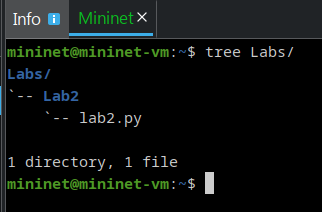
\includegraphics[height=7cm]{01} 
	\end{figure}
	
	Спочатку імпортуємо основні класи, потрібні для роботи. \texttt{Mininet} -- створює й керує емуляцією мережі (хости, свічі, лінки, контролери). \texttt{Controller} -- базовий (локальний) OpenFlow-контролер, \texttt{OVSSwitch} -- реалізація комутатора на базі Open vSwitch. CLI -- інтерактивна командна оболонка Mininet. Функція \texttt{setLogLevel} потрібна для встановлення рівеня логів (наприклад -- \texttt{info}). Імпорт стандартного модуля \texttt{os} використовується для виконання системних команд у хостовій VM.
	
	\begin{lstlisting}[language=Python]
		from mininet.net import Mininet 
		from mininet.node import Controller, OVSSwitch 
		from mininet.cli import CLI 
		from mininet.log import setLogLevel, info 
		import os\end{lstlisting}

	В головній функції \texttt{run} яка створює й запускає мережу, створюється об’єкт \texttt{net} типу Mininet. В параметрах вказується, що за замовчуванням використовується локальний контролер класу \texttt{Controller} та Open vSwitch як реалізація свічів.
	
	\begin{lstlisting}[language=Python]
		def run():
			net = Mininet(controller=Controller, switch=OVSSwitch)\end{lstlisting}
	
	Далі додамо контролер, свіч, хости (клієнти) та зв'язки між ними. Запустимо мережу.
	
	\begin{lstlisting}[language=Python]
		c0 = net.addController('c0')
		s1 = net.addSwitch('s1')
		h1 = net.addHost('h1', ip='10.0.0.1/24')
		h2 = net.addHost('h2', ip='10.0.0.2/24')
		h3 = net.addHost('h3', ip='10.0.0.3/24')
		
		net.addLink(h1, s1)
		net.addLink(h2, s1)
		net.addLink(h3, s1)
		
		net.start()\end{lstlisting}
	
	За замовчуванням OVS це L2-пристрій без IP-адреси. Щоб мати можливість надіслати пінг до OpenFlow-комутатора, зробити \texttt{traceroute}, або запускати інші діагностичні інструменти -- потрібно створити інтерфейс і дати йому ІР.
	
	\begin{lstlisting}[language=Python]
		info('*** Adding internal management port s1-mgmt with IP 10.0.0.254/24\n')
		os.system('ovs-vsctl add-port s1 s1-mgmt -- set interface s1-mgmt type=internal')
		
		os.system('ip addr add 10.0.0.254/24 dev s1-mgmt || true')
		os.system('ip link set s1-mgmt up || true')\end{lstlisting}
	
	Запускаємо на другому і третьому клієнті HTTP сервери в фоні (щоб скрипт не чекав завершення процесу).
	
	\begin{lstlisting}[language=Python]
		info('*** Starting HTTP servers on h2 and h3 (port 80)\n')
		h2.cmd('python3 -m http.server 80 &')
		h3.cmd('python3 -m http.server 80 &')\end{lstlisting}
	
	Запускаємо Mininet CLI -- інтерактивний інтерфейс, де можна виконувати команди на хостах. Після виходу з CLI (тобто після \texttt{CLI(net)}), викликається \texttt{net.stop()}, яка зупиняє мережу: вимикає контролер, свічі, видаляє інтерфейси й очищає ресурси.
	
	\begin{lstlisting}[language=Python]
		info('*** Setup complete - entering CLI\n')
		CLI(net)
		net.stop()\end{lstlisting}
	
	Наприкінці встановлюємо рівень логування Mininet на \texttt{info}, щоб бачити інформаційні повідомлення, статуси під час старту тощо, та викликаємо головну функцію \texttt{run()}, яка створює та керує мережею.
	
	\begin{lstlisting}[language=Python]
		if __name__ == "__main__":
			setLogLevel('info')
			run()\end{lstlisting}
		
	Виконуємо скрипт, перевіряємо стан мережі:
	
	\begin{figure}[H]
		\centering
		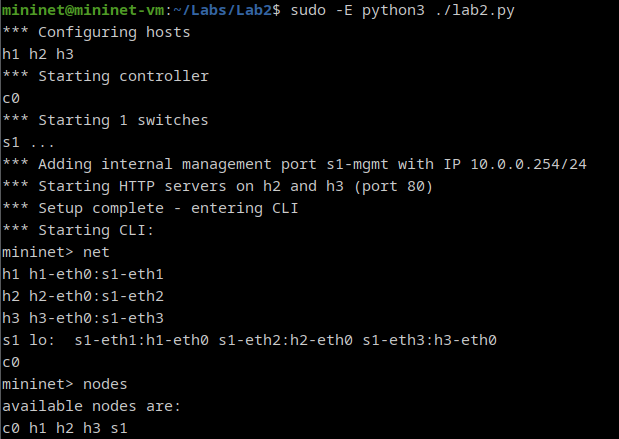
\includegraphics[height=10cm]{02} 
	\end{figure}
	
	Пінгуємо з основного клієнту (\texttt{h1}) сервери (\texttt{h2}, \texttt{h3}):
	
	\begin{figure}[H]
		\centering
		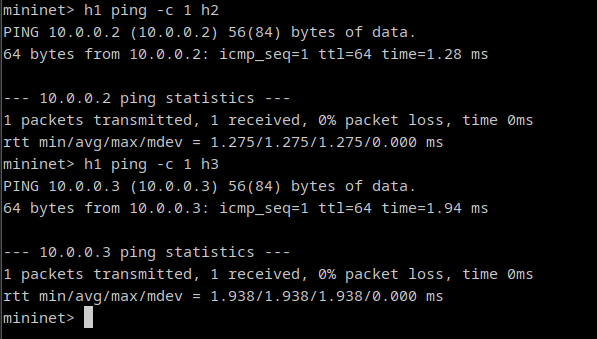
\includegraphics[height=10cm]{03} 
	\end{figure}
	
	Доступність HTML сторінок можна перевірити за допомогою утиліти \texttt{curl}:
	
	\begin{figure}[H]
		\centering
		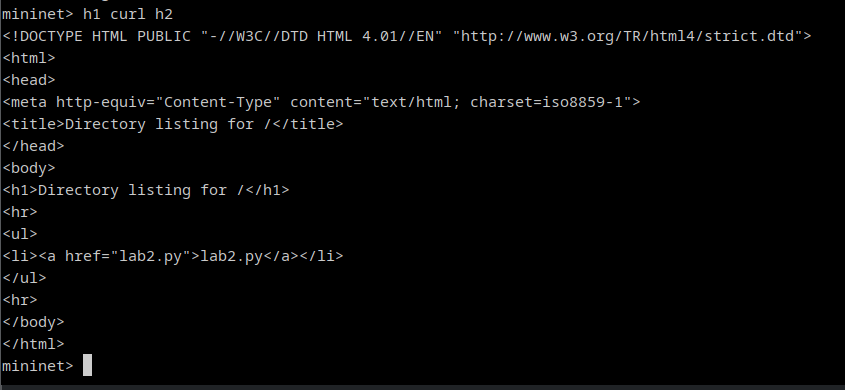
\includegraphics[height=8cm]{04} 
	\end{figure}
	
	Якщо ж команда не працює бо утиліта відсутня, її треба встановити на самій віртуальній машині, поза \texttt{mininet}. Так як хости працюють за допомогою механізму неймспейсів, то пакет буде доступним і там. Також треба встановити утиліту \texttt{traceroute} для подальшої роботи.
	
	\begin{figure}[H]
		\centering
		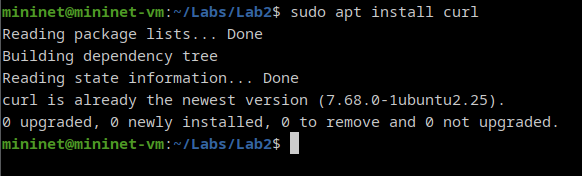
\includegraphics[height=5cm]{05} 
	\end{figure}
	
	Також, якщо додати прапорець "-І", можна дізнатися версію сервера, тощо. Це відбувається за допомогою перегляду заголовків пакету.
	
	\begin{figure}[H]
		\centering
		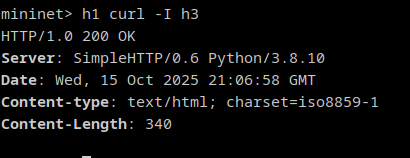
\includegraphics[height=6cm]{06} 
	\end{figure}
	
	
	Проведемо пінг та знаходження маршруту через комутатор.
	
	\begin{figure}[H]
		\centering
		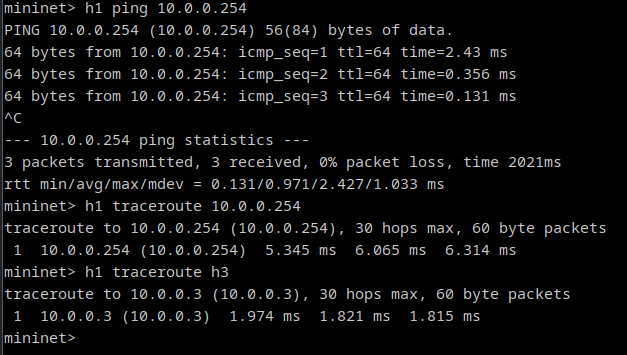
\includegraphics[height=9cm]{07} 
	\end{figure}
	
	Відсутність хопів можна пояснити тим, що це комутатор, а не маршрутизатор. Як бачимо, все працює.
	
	Насамкінець, спробуємо пропінгувати та дістати веб-сторінку з самої віртуальної машини Mininet, а не в середині CLI. Для цього під'єднаємося ще раз, з першого підключення запустимо скрипт, а з другого виконаємо операції (або ж просто можна запустити скрипт у фоні):
	
	\begin{figure}[H]
		\centering
		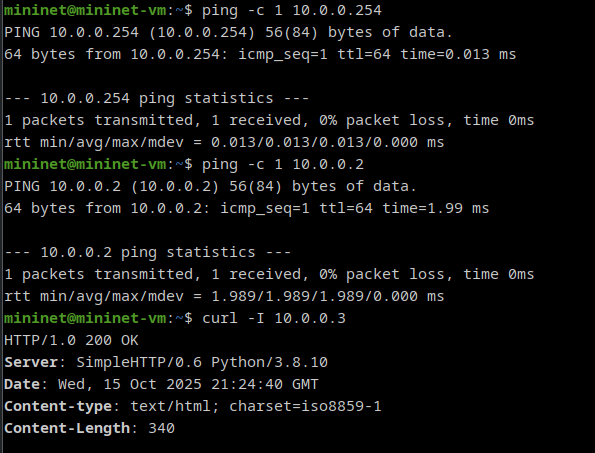
\includegraphics[height=11cm]{08} 
	\end{figure}
	
	Це спрацювало саме через те, що відповідний ІР був назначений в самому скрипті. Мережева конфігурація віртуальної машини представлена на скріншоті, де видно, що прямого доступу до ІР-адреси 10.0.0.3 немає.
	
	\begin{figure}[H]
		\centering
		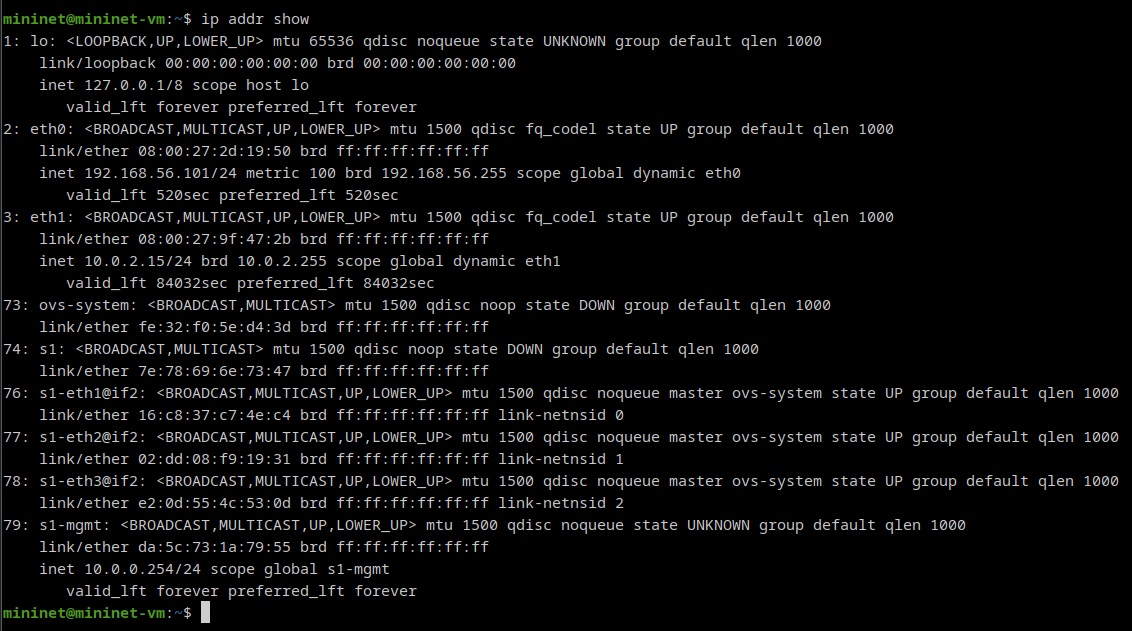
\includegraphics[height=10cm]{09} 
	\end{figure}
	
	Знаходження шляху також працює.
	
	\begin{lstlisting}[language=Bash]
		mininet@mininet-vm:~$ traceroute 10.0.0.2
		traceroute to 10.0.0.2 (10.0.0.2), 30 hops max, 60 byte packets
		1  10.0.0.2 (10.0.0.2)  1.435 ms  3.347 ms  3.371 ms\end{lstlisting}
	
	Додатково проведемо перевірку через утиліту \texttt{tcpdump}. На скріншоті можна побачити шлях пакету-запиту та пакету-відповіді. Це результат пінгу з консолі віртуальної машини до віртуального хосту \texttt{h2}, який має адресу \texttt{10.0.0.2}.
	
	\begin{figure}[H]
		\centering
		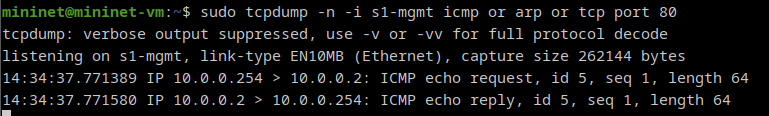
\includegraphics[height=2.7cm]{10} 
	\end{figure}
	
	\textbf{Висновок.}
	Під час виконання лабораторної роботи було успішно реалізовано просту SDN-мережу з одним клієнтом та двома HTTP-серверами за допомогою Mininet та Open vSwitch. Було написано і виконано Python-скрипт, який створює топологію, піднімає OVS-комутатор \texttt{s1}, підключає хости \texttt{h1}, \texttt{h2}, \texttt{h3}, додає internal-порт \texttt{s1-mgmt} з IP-адресою для менеджменту та запускає HTTP-сервери на \texttt{h2} і \texttt{h3}. За допомогою інструментів \texttt{ping}, \texttt{curl} та \texttt{tcpdump} перевірено доступність серверів і наявність трафіку. Також проведено експеримент з \texttt{traceroute}, який продемонстрував важливу відмінність між L2-комутатором і L3-маршрутизатором -- OVS як L2-пристрій не декрементує TTL, тому \texttt{traceroute} у даній плоскій топології показує один хоп.
	
	Результати роботи підтвердили виконання поставлених завдань і дозволили набути практичних навичок.
	
	\begin{center}
		\textbf{Лістинг скрипту.}
	\end{center}
	
	\begin{lstlisting}[language=Python]
		#!/usr/bin/env python3
		from mininet.net import Mininet
		from mininet.node import Controller, OVSSwitch
		from mininet.cli import CLI
		from mininet.log import setLogLevel, info
		import os
		
		def run():
			net = Mininet(controller=Controller, switch=OVSSwitch)
			c0 = net.addController('c0')
			s1 = net.addSwitch('s1')
			h1 = net.addHost('h1', ip='10.0.0.1/24')
			h2 = net.addHost('h2', ip='10.0.0.2/24')
			h3 = net.addHost('h3', ip='10.0.0.3/24')
		
			net.addLink(h1, s1)
			net.addLink(h2, s1)
			net.addLink(h3, s1)
		
			net.start()
		
			info('*** Adding internal management port s1-mgmt with IP 10.0.0.254/24\n')
			os.system('ovs-vsctl add-port s1 s1-mgmt -- set interface s1-mgmt type=internal')
		
			os.system('ip addr add 10.0.0.254/24 dev s1-mgmt || true')
			os.system('ip link set s1-mgmt up || true')
		
			info('*** Starting HTTP servers on h2 and h3 (port 80)\n')
			h2.cmd('python3 -m http.server 80 &')
			h3.cmd('python3 -m http.server 80 &')
		
			info('*** Setup complete - entering CLI\n')
			CLI(net)
			net.stop()
		
		if __name__ == "__main__":
			setLogLevel('info')
			run()\end{lstlisting}
		
\end{document}
